\documentclass[tikz]{standalone}
\usepackage{pgfplots}
\pgfplotsset{compat=1.15}
\usepackage{mathrsfs}
\usetikzlibrary{arrows,calc}
\usepackage{tkz-euclide}
\pagestyle{empty}

\definecolor{AngleClr}{rgb}{0,0.39215686274509803,0}
\definecolor{ShapeClr}{rgb}{0.6,0.2,0}

\begin{document}

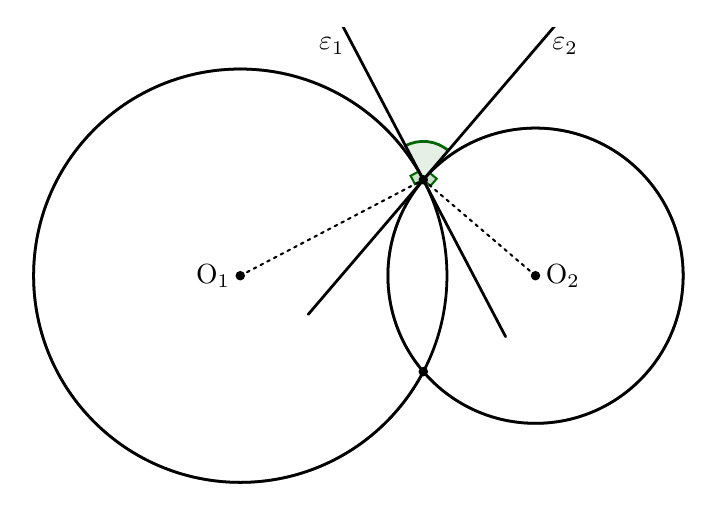
\begin{tikzpicture}[scale=.75]

\clip(-3.6,-3.6) rectangle (7.6,4.2);
\tkzSetUpLine[line width=1pt,color=black]
\tkzSetUpPoint[fill=black]

\tkzDefPoints{0/0/O1,5/0/O2,3.5/0/A,2.5/0/B}
\tkzDefPoints{1.55/4.2/E1,5.5/4.2/E2}

\tkzInterCC(O1,A)(O2,B) \tkzGetPoints{C}{D}
\tkzInterLL(O1,O2)(C,D) \tkzGetPoint{X}

\tkzDefLine[tangent at=C](O1) \tkzGetPoint{h1}
\tkzDefLine[tangent at=C](O2) \tkzGetPoint{H2}

\tkzDefPointOnLine[pos=-1](C,H2)\tkzGetPoint{h2}

\tkzDrawCircle[line width=1.0pt,fill=white](O1,A)
\tkzDrawCircle[line width=1.0pt,fill=white](O2,B)

\tkzDrawCircle[line width=1.0pt,color=black](O1,A)
\tkzDrawCircle[line width=1.0pt,color=black](O2,B)

\tkzFillAngle[fill=AngleClr,size=.65,fill opacity=0.1](h2,C,h1)
\tkzMarkAngle[line width=1pt,size=.65,color=AngleClr](h2,C,h1)

\tkzMarkRightAngles[line width=0.75pt, size=.16,color=AngleClr,fill=AngleClr,fill opacity=0.2](O1,C,h1 O2,C,h2)

% \tkzDrawSegments[line width=1pt,color=black](O1,O2 C,D)
\tkzDrawSegments[line width=1pt,color=black,add=3 and 3](C,h1 C,h2)
\tkzDrawSegments[line width=0.75pt,color=black,dashed,dash pattern=on 1pt off 1.75pt](O1,C O2,C)

\tkzDrawPoints[size=3](O1,O2,C,D) % ,TA,TB,TC,TD)
\tkzLabelPoint[left](O1){$\rm O_1$}
\tkzLabelPoint[right](O2){$\rm O_2$}
\tkzLabelPoint[below](E1){$\varepsilon_1$}
\tkzLabelPoint[below](E2){$\varepsilon_2$}


\end{tikzpicture}
\end{document}
